\section{Architecture overview}
\label{sec:architecture}

In this section we analyze the problem Disciplina aims to solve, describe the possible solutions and derive the architecture.

We start from some of the major requirements:

\begin{enumerate}
\item The platform should be able to store large quantities of private data such as grades, assignments, solutions, etc.
\item Educational institutions should be able to disclose the private data only to the payer.
\item The platform should guarantee fairness of the data trade without involving a third-party intermediary.
\end{enumerate}

Due to the nature of the platform, it has to operate on sensitive data, such as
courses, assignments, solutions and grades. Permissionless blockchains, like
Ethereum or EOS, would require disclosing this data to the public, whereas the
permissive ones, like Hyperledger, lack public verifiability.

It is important to note that it is possible to use encryption schemes in order to store sensitive information in public ledgers. This approach, despite being seemingly viable, suffers from incentive and scalability problems. The nodes of the blockchain would have to store every grade issued by all the educational institutions from all over the world. The expected size of the dataset exceeds the storage capacities of regular personal computers, which can lead to excessive centralization of the platform. Moreover, in most of the public ledgers the distributed storage is quite expensive, while there is no incentive for educaional institutions to pay for every grade they issue. Thus, we consider storing the educaitonal records on the public blockchain economically unjustified. What is more, it is hard to make the data disclosure process fair in such setting: in order to use the blockchain as an arbiter in case of dispute one has to reveal the encryption key to a subset of the transcrips issued by a certain educational institution.

Our architecture splits the blockchain into two layers: the private layer
contains sensitive data, and the public one contains the information necessary
to validate the integrity and authenticity of the private blocks. The key
entities of the proposed blockchain architecture are presented in
Figure~\ref{fig:entities}.

\begin{figure}[ht]
\centering
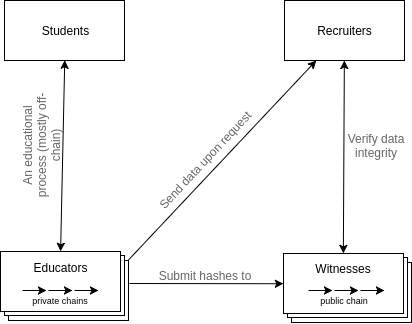
\includegraphics[width=0.7\textwidth]{entities-internal-storage}
\caption{Key entities of the Disciplina platform}
\label{fig:entities}
\end{figure}

The private layer is maintained by each Educator independently of others.
Educators can be either large educational institutes, capable of running their
own nodes, or some trusted party that runs the chain for the self-employed
teachers and small institutions. This layer contains the personalized
information on the interactions between the students and the Educator. All the
interactions, such as receiving an assignment, submitting solutions, or being
graded, are treated as transactions in the private chain.


Students get access to the platform through web and mobile applications. Using
the applications they choose Educators, enroll in courses, get assignments and
submit solutions. The scores and the criteria of whether the Student has
finished the course successfully are determined by the Educator. The education
process from the platform’s perspective is as follows:

\begin{enumerate}
\item A Student chooses an Educator and a course that she wants to enroll in.
\item If the course is offered on a pre-paid basis, the Student uses her app to
  pay the fee.
\item During the course, the Educator provides assignments that the Student has
  to complete in order to get the score.
\item The Student acquires the assignment, completes it and sends the signed
  solution back to the Educator (communication between the Student and the
  Educator happens off-chain).
\item The Educator then stores the solution locally, grades it with a score in
  range [0..100],  and transfers the score with the hash of the solution to the
  blockchain.
\item Upon the completion of the course, the Student acquires a final score
  based on the scores she got for her assignments. This final score is also
  added to the Educator’s chain.
\end{enumerate}

Making the Educators' chains private opens the possibility for Educators to
tamper with the data in their chains. To overcome this issue and make the
private transactions publicly verifiable, we introduce the second, public, layer
of the blockchain. The public part of the network consists of Witnesses –- the
special entities that witness the fact that a private block was produced by an
Educator.

They do so by writing the authentication information of a private block into the
public chain, which is used in the future by an arbitrary Verifier to
substantiate a proof of transaction inclusion given to it by a Student or an
Educator. Witnesses also process public information issued by the Educators,
such as announcements that an Educator has started or stopped offering a course
in a particular discipline. The Witnesses agree on which public blocks are valid
using the specified consensus rules.

The Recruiters are the entities interested in gathering data about students from
educational institutions. They buy this data from Educators using a secure data
disclosure protocol, described in detail in section \ref{sec:DataDisclosure}.
Validity and security of every data trade is also ensured by Witnesses, because
corresponding transactions and actions of each party are also stored in public
blockchain.
